% !TEX program = xelatex
% 因子特異性頻譜過濾下之廣義逆矩陣 Alpha — 碩士論文口試簡報
% 編譯：xelatex main.tex（執行兩次以定位校徽與標題列）
\documentclass[aspectratio=169,11pt,t]{beamer}   % t：內文靠上對齊（避免標題列下方留白過多）

\usepackage{fontspec}
\usepackage{amsmath}
\usepackage{unicode-math}
% ===== 拉丁字母與數學：Times New Roman =====
\setmainfont{Times New Roman}
\setmathfont{texgyretermes-math.otf}   % 與 Times 同字族的數學字型（以檔名載入）
\usepackage{xeCJK}
\usepackage{booktabs}
\usepackage{array}
\usepackage{colortbl}
\usepackage{graphicx}
\usepackage{tikz}
\usetikzlibrary{calc}

% ===== 中文字型：思源黑體 Noto Sans TC（系統實際安裝為同字形的 Noto Sans CJK TC）=====
\setCJKmainfont{Noto Sans CJK TC}
\setCJKsansfont{Noto Sans CJK TC}
\newCJKfontfamily\songti{Noto Sans CJK TC Medium}   % 標題頁與章節分隔頁（Medium 較有份量）
\newCJKfontfamily\heiti{Noto Sans CJK TC}

% ===== 政大配色 =====
\definecolor{nccublue}{RGB}{0,79,136}          % 標題列主色 #004F88（取自原簡報）
\definecolor{nccubluedk}{RGB}{0,56,100}
\definecolor{nccured}{RGB}{183,28,28}
\definecolor{ink}{RGB}{33,33,33}
\definecolor{softgray}{RGB}{120,120,120}

\graphicspath{{figs/}{assets/}}

% ===== Beamer 樣式 =====
\setbeamertemplate{navigation symbols}{}
\setbeamercolor{normal text}{fg=ink}
\setbeamercolor{frametitle}{fg=white,bg=nccublue}
\setbeamercolor{structure}{fg=nccublue}
\setbeamercolor{itemize item}{fg=ink}
\setbeamercolor{itemize subitem}{fg=ink}
\setbeamercolor{itemize subsubitem}{fg=ink}
\setbeamercolor{block title}{fg=white,bg=nccublue}
\setbeamercolor{block body}{bg=nccublue!6}

\setbeamertemplate{itemize item}{\small\raise0.15ex\hbox{$\bullet$}}
\setbeamertemplate{itemize subitem}{\small\raise0.10ex\hbox{$\circ$}}
\setbeamertemplate{itemize subsubitem}{\footnotesize\raise0.20ex\hbox{$\blacksquare$}}

\setbeamersize{text margin left=0.7cm,text margin right=0.7cm}

% ----- 標題列（政大藍滿版 + 右上校徽），永遠貼齊頂端 -----
\setbeamertemplate{frametitle}{%
  \begin{tikzpicture}[remember picture,overlay]
    \fill[nccublue] (current page.north west) rectangle ([yshift=-1.12cm]current page.north east);
    \node[anchor=west,text=white,inner sep=0pt] at ([xshift=0.55cm,yshift=-0.57cm]current page.north west)
      {\fontsize{17}{20}\selectfont\bfseries\insertframetitle};
    \node[anchor=south east,inner sep=0pt] at ([xshift=0cm,yshift=-1.12cm]current page.north east)
      {
\includegraphics[height=1.12cm]{nccu_logo.png}};
  \end{tikzpicture}%
  \vspace*{1.20cm}%
}

% ----- 章節分隔頁（藍列 + 校徽 + 置中宋體章名）-----
\newcommand{\chapterframe}[2]{%
  \begin{frame}[plain]
  \begin{tikzpicture}[remember picture,overlay]
    \fill[nccublue] (current page.north west) rectangle ([yshift=-1.12cm]current page.north east);
    \node[anchor=south east,inner sep=0pt] at ([xshift=0cm,yshift=-1.12cm]current page.north east)
      {
\includegraphics[height=1.12cm]{nccu_logo.png}};
    \node[align=center] at ([yshift=-0.3cm]current page.center)
      {\songti\fontsize{32}{40}\selectfont #1：#2};
  \end{tikzpicture}
  \end{frame}}

% ----- 小工具 -----
\newcommand{\hl}[1]{\textcolor{nccured}{\textbf{#1}}}     % 紅色強調數字
\newcommand{\figcap}[1]{\begin{center}\footnotesize\color{softgray}#1\end{center}}
\renewcommand{\arraystretch}{1.18}

\begin{document}

% ====================== 標題頁 ======================
\begin{frame}[plain]
\begin{tikzpicture}[remember picture,overlay]
  \node[rounded corners=16pt, fill=nccublue, text=white, align=center,
        inner xsep=26pt, inner ysep=20pt, text width=0.84\paperwidth] (titlebox)
       at ([yshift=1.0cm]current page.center)
       {{\songti\fontsize{25}{32}\selectfont 因子特異性頻譜過濾下之廣義逆矩陣 Alpha}\\[8pt]
        {\songti\fontsize{17}{23}\selectfont 台灣主動型股票基金之實證研究}};
  \node[anchor=north,align=center,text=ink] at ([yshift=-30pt]titlebox.south)
       {{\fontsize{15}{24}\selectfont 指導教授（Advisor）：羅秉政 博士}\\[12pt]
        {\fontsize{15}{24}\selectfont 研究生（Student）：胡益鳴\ 撰}};
\end{tikzpicture}
\end{frame}

% ====================== 大綱 ======================
\begin{frame}{大綱}
\vspace{0.4cm}
{\setbeamercolor{enumerate item}{fg=nccured}%
 \setbeamertemplate{enumerate item}{\color{nccured}\insertenumlabel.}%
 \large\color{nccured}
 \begin{enumerate}\setlength{\itemsep}{14pt}
   \item 緒論
   \item 文獻回顧與理論基礎
   \item 資料與研究方法
   \item 實證結果與分析
   \item 結論與未來展望
 \end{enumerate}}
\end{frame}

% ====================== 第一章 ======================
\chapterframe{第一章}{緒論}

\begin{frame}{緒論 — 研究背景與動機}
\vspace{0.2cm}
被動投資（0050 ETF）盛行，引發「主動管理是否仍具價值」的辯論。基金\textbf{持股明細}隱含經理人的私有資訊，但直接「跟單」在台灣面臨三大結構性挑戰：
\begin{itemize}\setlength{\itemsep}{8pt}
  \item \textbf{資訊遞延與前視偏誤}：季報公告落差達 60 天，投資人看到的是「舊聞」，跟單常買在經理人獲利了結之後。
  \item \textbf{維度災難}：股票數遠多於基金數（$N \gg M$），回歸矩陣\textbf{秩不足}，傳統 OLS 在數學上完全失效。
  \item \textbf{羊群效應與雜訊}：機構持股充斥追逐熱門股的從眾行為，難以區分「真實選股實力」與「盲目跟風」，信噪比過低。
\end{itemize}
\vspace{4pt}
\hfill{\small\color{softgray}$\Rightarrow$ 本研究以 Wermers et al. (2012) GIA 模型為基礎，發展「因子特異性參數校準」加以解決。}
\end{frame}

\begin{frame}{緒論 — 研究目的}
\vspace{0.3cm}
本研究檢驗廣義逆矩陣 Alpha（GIA）模型於台灣股票市場之選股效力，具體目的有三：
\begin{enumerate}\setlength{\itemsep}{12pt}
  \item \textbf{解決維度災難}：以奇異值分解（SVD）與截斷技術克服 $N \gg M$ 之數學限制，從持股共識中逆解個股預期超額報酬。
  \item \textbf{驗證因子頻譜結構}：探討不同屬性因子（共識型 vs.\ 私有型）在奇異值頻譜上是否呈現相異物理結構，並建立\textbf{因子特異性校準}機制以優化信噪比。
  \item \textbf{建構可獲利策略}：在資訊遞延下，檢驗 GIA 能否萃取具預測力的訊號，並在扣除交易成本與風險調整後，創造顯著優於 0050 ETF 的實質績效。
\end{enumerate}
\end{frame}

\begin{frame}{緒論 — 研究貢獻}
\vspace{0.25cm}
\begin{itemize}\setlength{\itemsep}{11pt}
  \item \textbf{方法論創新}：打破過往文獻（如 Wermers et al., 2012）「固定截斷參數」之限制，實證證明不同因子有截然不同的奇異值頻譜，需\textbf{差異化頻譜過濾}。
  \item \textbf{實證發現}：揭示資訊遞延導致的「歸因錯置」—— 高 Return Gap 隱含經理人已獲利了結，使該指標在台股轉為\hl{反向訊號}（$t=-2.51$）；經方向校準後轉為有效獲利來源。
  \item \textbf{實務價值}：即使扣除贏家策略高換股率衍生的成本，GIA 贏家組淨報酬（\hl{17.95\%}）仍遠勝被動大盤（12.18\%），為量化基金提供高 Alpha 多頭篩選引擎。
\end{itemize}
\end{frame}

% ====================== 第二章 ======================
\chapterframe{第二章}{文獻回顧與理論基礎}

\begin{frame}{文獻回顧 — 主動管理指標與羊群效應}
\vspace{0.2cm}
\begin{itemize}\setlength{\itemsep}{7pt}
  \item \textbf{歷史 Alpha 預測力衰減}：Jones and Mo (2021) 證實多數預測因子樣本外預測力顯著衰減（Alpha Spread 降幅過半），單靠歷史淨值回歸難以持續創造超額報酬。
  \item \textbf{主動份額（Active Share）}：Cremers and Petajisto (2009) 以持股差異區分「秘密指數者」與真正主動經理人；盧秋玲等 (2017) 在台灣驗證高 AS 基金扣費後選股能力較佳。
  \begin{itemize}\item \textbf{侷限}：AS 僅衡量「偏離程度」，無法判斷是否基於\textbf{正確的私有資訊}。\end{itemize}
  \item \textbf{羊群效應}：李春安與賴藝文 (2005) 發現台灣機構（尤以投信）在劇烈波動期存在顯著從眾行為，盲目跟單可能僅是從眾結果而非私有資訊，承擔過度擁擠風險。
\end{itemize}
\end{frame}

\begin{frame}{文獻回顧 — 廣義逆矩陣（GIA）之理論架構}
\vspace{0.2cm}
\begin{itemize}\setlength{\itemsep}{9pt}
  \item \textbf{選股能力的逆向工程}：Cohen, Coval, and Pástor (2005) 提出 Stock Quality —— 若能識別高能力經理人，其重倉股即為高品質股；個股 Alpha 可由持有它的經理人能力加權推導。
  \item \textbf{OLS 的維度失效}：金融市場 $N \gg M$，使 $W^{\top}W$ 秩不足、奇異不可逆，為欠定系統、存在無限多解，傳統 OLS 在數學定義上完全失效。
  \item \textbf{SVD 降維與頻譜過濾}：Wermers, Yao, and Zhao (2012) 引入\textbf{截斷奇異值分解}執行「頻譜過濾」—— 保留代表聰明錢共識的主成分、剔除尾端隨機交易雜訊，完美解決矩陣不可逆限制。
\end{itemize}
\end{frame}

\begin{frame}{文獻回顧 — 9 大績效預測因子總覽}
\vspace{-0.15cm}
本研究參考新興市場文獻（Li and Rao, 2023；Jones and Mo, 2021），選取 9 項廣受驗證之因子，依經濟意涵分三類：
\vspace{4pt}
\begin{center}\small
\begin{tabular}{>{\raggedright\arraybackslash}p{2.9cm} >{\raggedright\arraybackslash}p{8.8cm}}
\toprule
\textbf{類別} & \textbf{因子（代表文獻）} \\
\midrule
持股特徵結構 & 主動份額 AS（Cremers \& Petajisto, 2009）、持股廣度／集中度（Kacperczyk et al., 2005；Pollet \& Wilson, 2008） \\
歷史績效與風險 & 傳統 Alpha（Jensen 1968；Carhart 1997）、持股 Alpha（Wermers 2000；Elton et al., 2011）、主動風險 $1-R^2$（Amihud \& Goyenko, 2013）、追蹤誤差 TE（Cremers \& Petajisto, 2009） \\
交易行為與動能 & 持股動能 HBM（Grinblatt et al., 1995）、交易動能（Chen et al., 2000）、回報缺口 Return Gap（Kacperczyk et al., 2008） \\
\bottomrule
\end{tabular}
\end{center}
\vspace{2pt}
\hfill{\small\color{softgray}各因子之台灣在地化定義調整詳見第三章。}
\end{frame}

\begin{frame}{文獻回顧 — 研究缺口與本研究定位}
\vspace{0.3cm}
\begin{itemize}\setlength{\itemsep}{11pt}
  \item \textbf{方法論缺口}：台灣持股矩陣高度稀疏、秩不足，國內極少探討如何以數學降維（SVD）系統性解決維度災難並萃取訊號。
  \item \textbf{指標缺口}：國內多聚焦顯性特徵（AS、集中度），對計算複雜、捕捉「隱藏操作／純選股」的隱含指標（Holding Alpha、Return Gap）在散戶比例高的淺碟市場缺乏在地驗證。
  \item \textbf{整合性缺口}：過往多檢驗「單一因子」，少將持股結構、歷史績效與交易動能納入同一整合模型。本研究以 GIA 加權機制進行 9 大因子綜合分析。
\end{itemize}
\end{frame}

% ====================== 第三章 ======================
\chapterframe{第三章}{資料與研究方法}

\begin{frame}{研究資料、樣本與前視偏誤防範}
\vspace{0.1cm}
\begin{columns}[T]
\begin{column}{0.62\textwidth}
\small
\begin{itemize}\setlength{\itemsep}{6pt}
  \item \textbf{資料}：台灣經濟新報（TEJ）；期間 2006/01–2025/06，涵蓋金融海嘯、歐債、COVID-19 與升息循環之完整多空週期。
  \item \textbf{樣本篩選}：限 AA1 國內主動型股票基金，排除海外／平衡／固收／被動 ETF；回溯清算下市基金以\textbf{消除存續者偏誤}。
  \item \textbf{資訊對齊}：持股遞延一季（用 $t{-}1$ 季持股算 $t$ 季 GIA），杜絕前視偏誤；績效類因子用至 $t$ 季可得報酬。
  \item \textbf{流動性濾網}：排除季底收盤價 $<$ 10 元之雞蛋水餃股。
\end{itemize}
\end{column}
\begin{column}{0.38\textwidth}
\centering
\vspace{0.4cm}
\footnotesize
\textbf{表 1\ \ 樣本概況}\\[4pt]
\begin{tabular}{lc}
\toprule
項目 & 數量 \\
\midrule
基金總數 & 174 檔 \\
基金-年月觀測 & 278,837 \\
季平均基金數 & 106 檔 \\
季平均合規股票 & 353 檔 \\
\bottomrule
\end{tabular}
\end{column}
\end{columns}
\end{frame}

\begin{frame}{因子建構（1/4）— 持股結構}
\vspace{-0.05cm}\small
共同點：所有涉及持股的因子皆\textbf{遞延一季}（用 $t{-}1$ 季持股），避免前視偏誤。
\begin{itemize}\setlength{\itemsep}{8pt}
  \item \textcolor{nccublue}{\textbf{主動份額 Active Share（AS）}}：衡量持股「偏離同業共識」的程度——偏離越大，越敢獨立選股、越可能握有私有資訊。
  \[ AS_{f,t}=\tfrac{1}{2}\sum_{i=1}^{N}\bigl|\,w_{f,i,t-1}-w_{peer,i,t-1}\,\bigr| \]
  {\footnotesize\color{softgray} $w_{f,i,t-1}$：基金 $f$ 上季持股 $i$ 的權重；$w_{peer,i,t-1}$：該股在全體主動基金的平均權重。\textbf{台灣改良}：基準改用「同業平均」而非大盤，排除台積電權重過高造成的假性 AS。}
  \item \textcolor{nccublue}{\textbf{持股廣度 Diversification（DIV）}}：以持股檔數的對數作為「基金規模」的純淨代理。
  \[ DIV_{f,t}=\ln\!\bigl(N_{f,t-1}\bigr) \]
  {\footnotesize\color{softgray} $N_{f,t-1}$：上季持股總檔數。改用檔數而非 TNA，避免牛市市值「虛胖」混入 Beta；台股實證\textbf{檔數越多績效越好}（與歐美相反）。}
\end{itemize}
\end{frame}

\begin{frame}{因子建構（2/4）— 歷史績效（選股能力）}
\vspace{0.0cm}\small
兩項皆對 Carhart 四因子做 \textbf{36 個月}滾動迴歸取截距（視窗依 Jones \& Mo, 2021 最佳信噪比）。
\begin{itemize}\setlength{\itemsep}{9pt}
  \item \textcolor{nccublue}{\textbf{傳統基金 Alpha}}：用基金\textbf{實際淨值月報酬}迴歸，截距 $\alpha_f$ 即扣除費用與系統性風險後的真實超額報酬。
  \[ R_{f,t}-RF_t=\alpha_f+\beta_1 MKT_t+\beta_2 SMB_t+\beta_3 HML_t+\beta_4 MOM_t+\epsilon_t \]
  \item \textcolor{nccublue}{\textbf{持股 Alpha（Holding Alpha）}}：改用「季初持股回推的\textbf{買入持有報酬} $R_{H,f,t}$」做同樣迴歸，截距 $\alpha_{H,f}$。
  \[ R_{H,f,t}-RF_t=\alpha_{H,f}+\beta_1 MKT_t+\beta_2 SMB_t+\beta_3 HML_t+\beta_4 MOM_t+\epsilon_t \]
  {\footnotesize\color{softgray} 排除了費用與現金拖累（Cash Drag），反映更純粹的基本面選股技巧。}
\end{itemize}
\end{frame}

\begin{frame}{因子建構（3/4）— 主動風險（主動程度）}
\vspace{0.1cm}\small
此兩項從「風險」角度驗證經理人是否真正偏離大盤、具備穩定的主動風格。
\begin{itemize}\setlength{\itemsep}{11pt}
  \item \textcolor{nccublue}{\textbf{主動風險 $1-R^2$}}（Amihud \& Goyenko, 2013）：取四因子迴歸的判定係數 $R^2$；$1-R^2$ 即報酬中「無法被市場因子解釋」的特異比例，越高代表越靠獨立選股、越不隨波逐流。
  \[ ActiveRisk_{f,t}=1-R^2_{f,t} \]
  \item \textcolor{nccublue}{\textbf{追蹤誤差 Tracking Error（TE）}}：主動報酬（相對大盤超額報酬）的波動標準差，衡量主動操作承擔的風險。
  \[ TE_{f,t}=\sqrt{\tfrac{1}{11}\sum_{k=t-11}^{t}\bigl(e_{f,k}-\overline{e_f}\bigr)^2},\qquad e_{f,k}=(R_{f,k}-RF_k)-MKT_k \]
  {\footnotesize\color{softgray} 視窗用 \textbf{12 個月}（台股產業風格轉換快，需較靈敏地捕捉短期主動暴露）。}
\end{itemize}
\end{frame}

\begin{frame}{因子建構（4/4）— 交易行為與動能}
\vspace{-0.15cm}\small
\setlength\abovedisplayskip{2pt}\setlength\belowdisplayskip{2pt}
動能視窗採 \textbf{6 個月}（台股電子業循環短、輪動快，需反應靈敏）。$Ret_{i,t-6\to t}$：股票 $i$ 過去 6 個月累積報酬。
\begin{itemize}\setlength{\itemsep}{2pt}
  \item \textcolor{nccublue}{\textbf{持股動能 HBM（存量）}}：當下持股「是否由過去贏家股構成」——以持股權重對個股動能加權。
  \[ HBM_{f,t}=\sum_{i=1}^{N}\bigl(w_{f,i,t-1}\times Ret_{i,t-6\to t}\bigr) \]
  \item \textcolor{nccublue}{\textbf{交易動能 TradingMoM（流量）}}：經理人是「加碼」還是「減碼」贏家股——以權重\textbf{變動量}對動能加權。
  \[ TradingMoM_{f,t}=\sum_{i=1}^{N}\bigl(w_{f,i,t-1}-w_{f,i,t-2}\bigr)\times Ret_{i,t-6\to t} \]
  \item \textcolor{nccublue}{\textbf{回報缺口 Return Gap}}：基金實際報酬 $-$ 用上季持股「靜態推算」的報酬；正值代表季中隱藏交易（波段操作）創造了額外價值。
  \[ GAP_{f,t}=R_{f,t}-\sum_{i=1}^{N}\bigl(w_{f,i,t-1}\times R_{i,t}\bigr) \]
\end{itemize}
\end{frame}

\begin{frame}{GIA 模型核心邏輯與 OLS 失效}
\vspace{0.25cm}
\textbf{逆向工程}：已知基金能力向量 $\hat S$（9 大因子分數）與持股權重矩陣 $W$，反推未知的個股預期超額報酬向量 $\alpha$，建立線性模型：
\[ \hat S = W\alpha + e \]
\vspace{-4pt}
\begin{itemize}\setlength{\itemsep}{7pt}
  \item $\hat S$：$M\times 1$ 基金能力向量；\quad $W$：$M\times N$ 持股權重矩陣；\quad $\alpha$：$N\times 1$ 待解個股 Alpha。
  \item \textbf{維度災難}：台股 $N \gg M$，$W^{\top}W$ 秩不足（$\mathrm{Rank}\le M < N$）、行列式為零 $\Rightarrow$ 反矩陣不存在。
  \item 此欠定系統存在無限多解，傳統 OLS \textbf{在數學定義上完全失效}。
\end{itemize}
\end{frame}

\begin{frame}{奇異值分解（SVD）與三階段資訊傳遞（1/2）}
\vspace{0.15cm}
將持股權重矩陣分解為三個矩陣： \quad $W = U\Sigma V^{\top}$
\vspace{4pt}

{\small\textcolor{nccublue}{\textbf{直覺}}：分解後會浮現幾個隱含的「投資風格」——同一個風格（如電子成長），\textbf{$U$ 看「哪些基金」屬於它、$V$ 看「哪些股票」屬於它}，$\Sigma$ 看它有多主流。}
\vspace{6pt}
\begin{itemize}\setlength{\itemsep}{8pt}
  \item $U$（\textbf{基金特徵空間}）：$M\times M$ 正交矩陣，捕捉基金之間的風格相似性。
  \item $\Sigma$（\textbf{訊息強度}）：對角奇異值 $\sigma_1\ge\sigma_2\ge\cdots\ge0$，代表各風格因子在持股結構中的重要性。
  \item $V$（\textbf{股票特徵空間}）：$N\times N$ 正交矩陣，捕捉個股之間的「共同持有模式」—— 常被同一群基金持有的股票，共享隱含投資屬性。
\end{itemize}
\end{frame}

\begin{frame}{奇異值分解（SVD）與三階段資訊傳遞（2/2）}
\vspace{0.0cm}
\setlength\abovedisplayskip{2pt}\setlength\belowdisplayskip{2pt}
\[ \hat\alpha_{GIA}=W^{+}\hat S = V\,\Sigma_K^{+}\,U^{\top}\hat S \]
\begin{itemize}\setlength{\itemsep}{2pt}
  \item \textbf{風格歸因}（$U^{\top}\hat S$）：將績效投影至基金空間，把「誰賺錢」轉化為「哪種風格賺錢」。
  \item \textbf{去跟風化校準}（$\Sigma_K^{+}$）：\textbf{大奇異值}＝多數基金擁擠的共識交易，以 $1/\sigma_i$ 縮小權重、剝離羊群順風車；\textbf{中等奇異值}＝少數經理人獨有的選股，保留其訊號；\textbf{尾端微小奇異值}＝隨機雜訊，強制清零。
  \item \textbf{映射至個股}（$V$）：把校準後的純淨風格 Alpha，依「每檔股票與各風格的關聯程度」分配回個股，形成最終個股 GIA 分數。
\end{itemize}
\vspace{-2pt}
\begin{block}{與 Stock Quality（Cohen et al., 2005）的關係}
\footnotesize $W$ 各列向量正交＝\textbf{各基金持股完全不重疊}，此時 GIA 退化為簡單加權 $\hat\alpha\propto W^{\top}\hat S$（即 Stock Quality）。但持股不可能不重疊——簡單加權會讓「被越多基金共同持有」的股票被灌水（\textbf{誤把擁擠當品質}）；GIA 以 $V\Sigma_K^{+}U^{\top}$ 校正重疊、剝離羊群，這正是其優勢。
\end{block}
\end{frame}

\begin{frame}{本文核心創新 — 因子特異性頻譜過濾}
\vspace{0.1cm}
\small 過往文獻多用固定截斷 $K=M/2$，隱含「所有因子資訊衰減相同」。本研究依因子物理特性動態校準：
\[ \Sigma_K^{+(i,i)}=
\begin{cases} 1/\sigma_i, & i\le K \quad(\text{保留主要訊息})\\[2pt] 0, & i> K \quad(\text{過濾雜訊，避免發散})\end{cases} \]
\begin{itemize}\setlength{\itemsep}{5pt}
  \item \textbf{廣泛共識型}（如 HBM）：訊息散布全市場共同持有模式，需保留高比例頻譜，最適 $K\approx 0.95$。
  \item \textbf{稀疏訊號型}（如 Return Gap）：私有資訊高度集中於前幾個主成分，餘皆雜訊，需嚴格過濾 $K\approx 0.3$。
  \item \textbf{標準結構型}（如 Holding Alpha、AS）：訊噪均衡衰減，最適落在 $K\in[0.4,0.6]$，呼應 Wermers et al.\ $K\approx M/2$。
\end{itemize}
\end{frame}

\begin{frame}{回測架構與績效評估指標}
\vspace{0.15cm}
\small
\begin{itemize}\setlength{\itemsep}{6pt}
  \item \textbf{投組建構}：每季依 GIA 分數排序等分 10 組（Decile）；$t$ 季底成形、$t{+}1$ 季第一個交易日建倉並持有整季。
  \item \textbf{等權重配置}：台股市值集中台積電，市值加權會被權值股 Beta 主導；等權重以檢驗在各規模區間皆具普遍選股力。
  \item \textbf{多空策略}：$R_{L/S,t+1}=R_{D10,t+1}-R_{D1,t+1}$（零成本，原始報酬以純測訊號強度）。
  \item \textbf{統計檢定}：Newey-West HAC（lags = 4）修正序列相關與異質變異；Spearman 單調性檢定。
  \item \textbf{兩階段策略}：① 單因子結構驗證與 $K$ 敏感度分析；② 多因子等權整合（1/N；DeMiguel et al., 2009）避免過度擬合。
\end{itemize}
\end{frame}

% ====================== 第四章 ======================
\chapterframe{第四章}{實證結果與分析}

\begin{frame}{單因子 GIA、頻譜校準與兩階段篩選}
\vspace{-0.1cm}
\footnotesize
\begin{columns}[T]
\begin{column}{0.99\textwidth}
\centering
\textbf{表 2\ \ 單因子績效與篩選決策表}\\[3pt]
\begin{tabular}{l l c c c c l}
\toprule
因子 & 結構分類 & $K^{*}$ & 多空季均 & $t$ 值 & Spearman $\rho$ & 篩選決策 \\
\midrule
HBM            & Consensus & 0.95 & 2.78\% & 3.09 & 0.794 & 納入（核心動能） \\
TradingMoM     & Standard  & 0.65 & 2.64\% & 3.50 & 0.697 & 納入（交易動能） \\
TrackingError  & Standard  & 0.60 & 0.90\% & 1.89 & 0.600 & 納入（架構濾網） \\
Active Share   & Standard  & 0.50 & 1.20\% & 1.90 & 0.539 & 納入（架構濾網） \\
OneMinusR2     & Standard  & 0.50 & 1.57\% & 4.01 & 0.697 & 納入（選股能力） \\
Holding Alpha  & Standard  & 0.50 & 1.95\% & 2.60 & 0.370 & \textcolor{nccured}{排除（單調性弱）} \\
Diversification& Standard  & 0.40 & 1.49\% & 2.37 & 0.649 & \textcolor{nccured}{排除（冗餘）} \\
TraditionalAlpha& Standard & 0.50 & $-$0.44\% & $-$0.78 & $-$0.309 & \textcolor{nccured}{排除（不顯著）} \\
ReturnGap      & Sparse    & 0.30 & $-$1.82\% & $-$2.51 & $-$0.673 & 納入（反向指標） \\
\bottomrule
\end{tabular}
\end{column}
\end{columns}
\vspace{5pt}
\scriptsize
\textbf{兩階段篩選}：① 顯著性 —— 剔除不顯著的 Traditional Alpha；② 效率／冗餘 —— 剔除單調性弱的 Holding Alpha（$\rho=0.37$）；剔除 Diversification（與 AS／$1-R^2$ 資訊重疊、都是在衡量集中度，於既有因子下無顯著邊際貢獻且拉低 Sharpe）。最終鎖定 \hl{6 大核心因子}（HBM、TradingMoM、Return Gap、$1-R^2$、Active Share、TE）。
\end{frame}

\begin{frame}{基金層級驗證 — GIA 的跨層級資訊轉換價值}
\vspace{0.1cm}
\small 比較「基金層級」與「GIA 反推之股票層級」結果，多項因子\textbf{預測力顯著不一致}：
\vspace{3pt}
\begin{center}\footnotesize
\begin{tabular}{l c c >{\raggedright\arraybackslash}p{5.2cm}}
\toprule
因子 & 基金層級 & GIA 股票層級 & 啟示 \\
\midrule
OneMinusR2 & $\rho\approx0$（$p=0.96$） & $t=4.01,\ \rho=0.70$ & 基金層級幾無預測力，經 SVD 後浮現強訊號 \\
Return Gap & $+0.71$（正向） & $t=-2.51$（翻負） & 資訊遞延導致訊號反轉（歸因錯置） \\
Holding Alpha & $0.90$（次強） & $\rho=0.37$（弱化） & 單調性不足，故於整合階段剔除 \\
\bottomrule
\end{tabular}
\end{center}
\vspace{5pt}
\begin{block}{方法論意涵}
\small GIA \textbf{並非}基金層級訊號的簡單加權平均，而是透過 SVD 頻譜過濾，從持股共現模式中萃取出「相對於基金層級具獨立預測力」的股票層級 Alpha —— 這正是採用 GIA 而非簡單加權法的正當性所在。
\end{block}
\end{frame}

\begin{frame}{整合 GIA 投資組合 — 分組績效（單調性）}
\vspace{0.15cm}
\begin{columns}[c]
\begin{column}{0.62\textwidth}
\centering
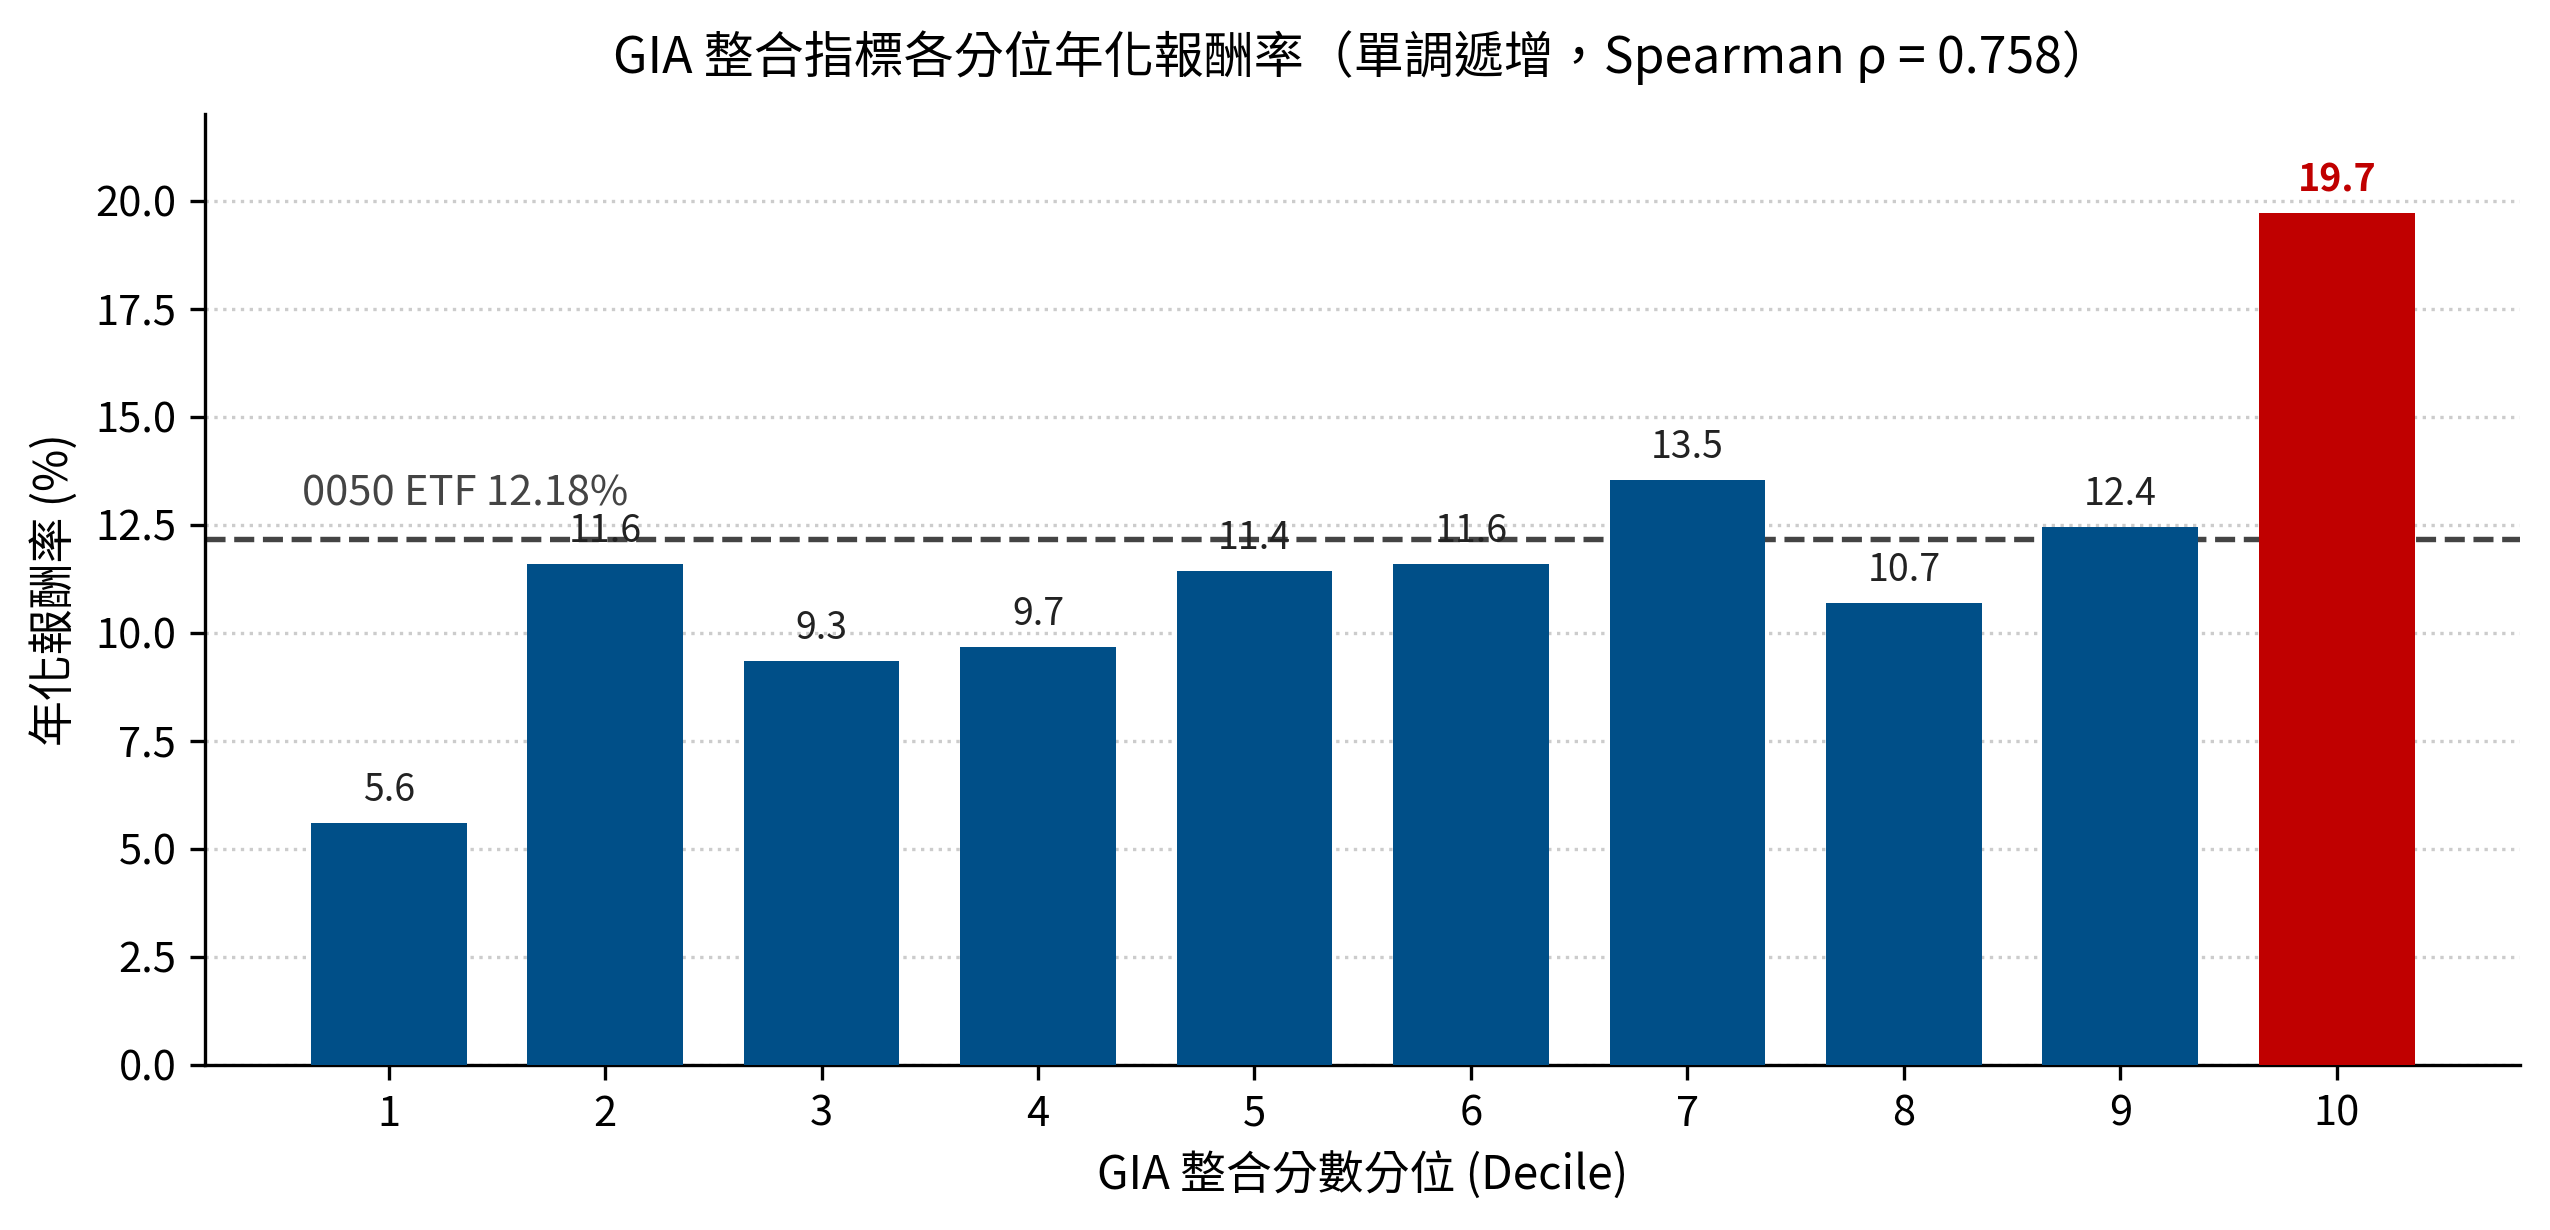
\includegraphics[width=\linewidth]{decile_bar.png}
\end{column}
\begin{column}{0.37\textwidth}
\small
\begin{itemize}\setlength{\itemsep}{8pt}
  \item 6 因子等權整合（負向因子先做\textbf{方向校準} $\times(-1)$）。
  \item 年化報酬由 D1（\hl{5.6\%}）單調遞增至 D10（\hl{19.72\%}）。
  \item Spearman $\rho=\hl{0.758}$（$p=0.011$），具顯著單調遞增特性。
\end{itemize}
\end{column}
\end{columns}
\figcap{資料來源：本研究實證結果（表 4）。虛線為 0050 ETF 年化報酬 12.18\%。}
\end{frame}

\begin{frame}{整合 GIA 投資組合 — 分組績效表}
\vspace{-0.02cm}
\renewcommand{\arraystretch}{1.04}
\footnotesize
\begin{center}
\textbf{表 4\ \ GIA 整合指標分組績效表（2006Q1–2025Q2）}\\[4pt]
\begin{tabular}{c c c c c c}
\toprule
分組 & 年化報酬 & $t$ 值 & 年化波動 & 夏普比率 & 最大回撤 \\
\midrule
1 (輸家) & 5.60\%  & 1.03 & 22.65\% & 0.247 & $-$61.54\% \\
2 & 11.59\% & 1.93 & 23.76\% & 0.488 & $-$63.61\% \\
3 & 9.35\%  & 1.67 & 23.20\% & 0.403 & $-$60.50\% \\
4 & 9.66\%  & 1.80 & 22.72\% & 0.425 & $-$58.06\% \\
5 & 11.44\% & 2.06 & 22.71\% & 0.504 & $-$62.57\% \\
6 & 11.59\% & 2.35 & 23.06\% & 0.503 & $-$59.43\% \\
7 & 13.53\% & 2.23 & 24.17\% & 0.560 & $-$68.30\% \\
8 & 10.69\% & 2.00 & 22.73\% & 0.470 & $-$65.65\% \\
9 & 12.44\% & 2.20 & 23.29\% & 0.534 & $-$64.30\% \\
\rowcolor{nccublue!12}\textbf{10 (贏家)} & \textbf{19.72\%} & \textbf{3.05} & 26.40\% & \textbf{0.747} & $-$64.95\% \\
\rowcolor{nccured!10}\textbf{L/S} & \textbf{14.12\%} & \textbf{4.71} & \textbf{13.70\%} & \textbf{1.031} & \textbf{$-$17.39\%} \\
\bottomrule
\end{tabular}
\end{center}
\vspace{3pt}
\scriptsize\color{softgray} 多空原始利差 $t=4.71$ 遠高於 1\% 臨界值 2.58；L/S 波動僅 13.70\%、MDD 僅 $-17.39\%$，顯示因子本身具良好對沖避險能力。
\end{frame}

\begin{frame}{累積報酬走勢}
\vspace{0.1cm}
\begin{columns}[c]
\begin{column}{0.70\textwidth}
\centering
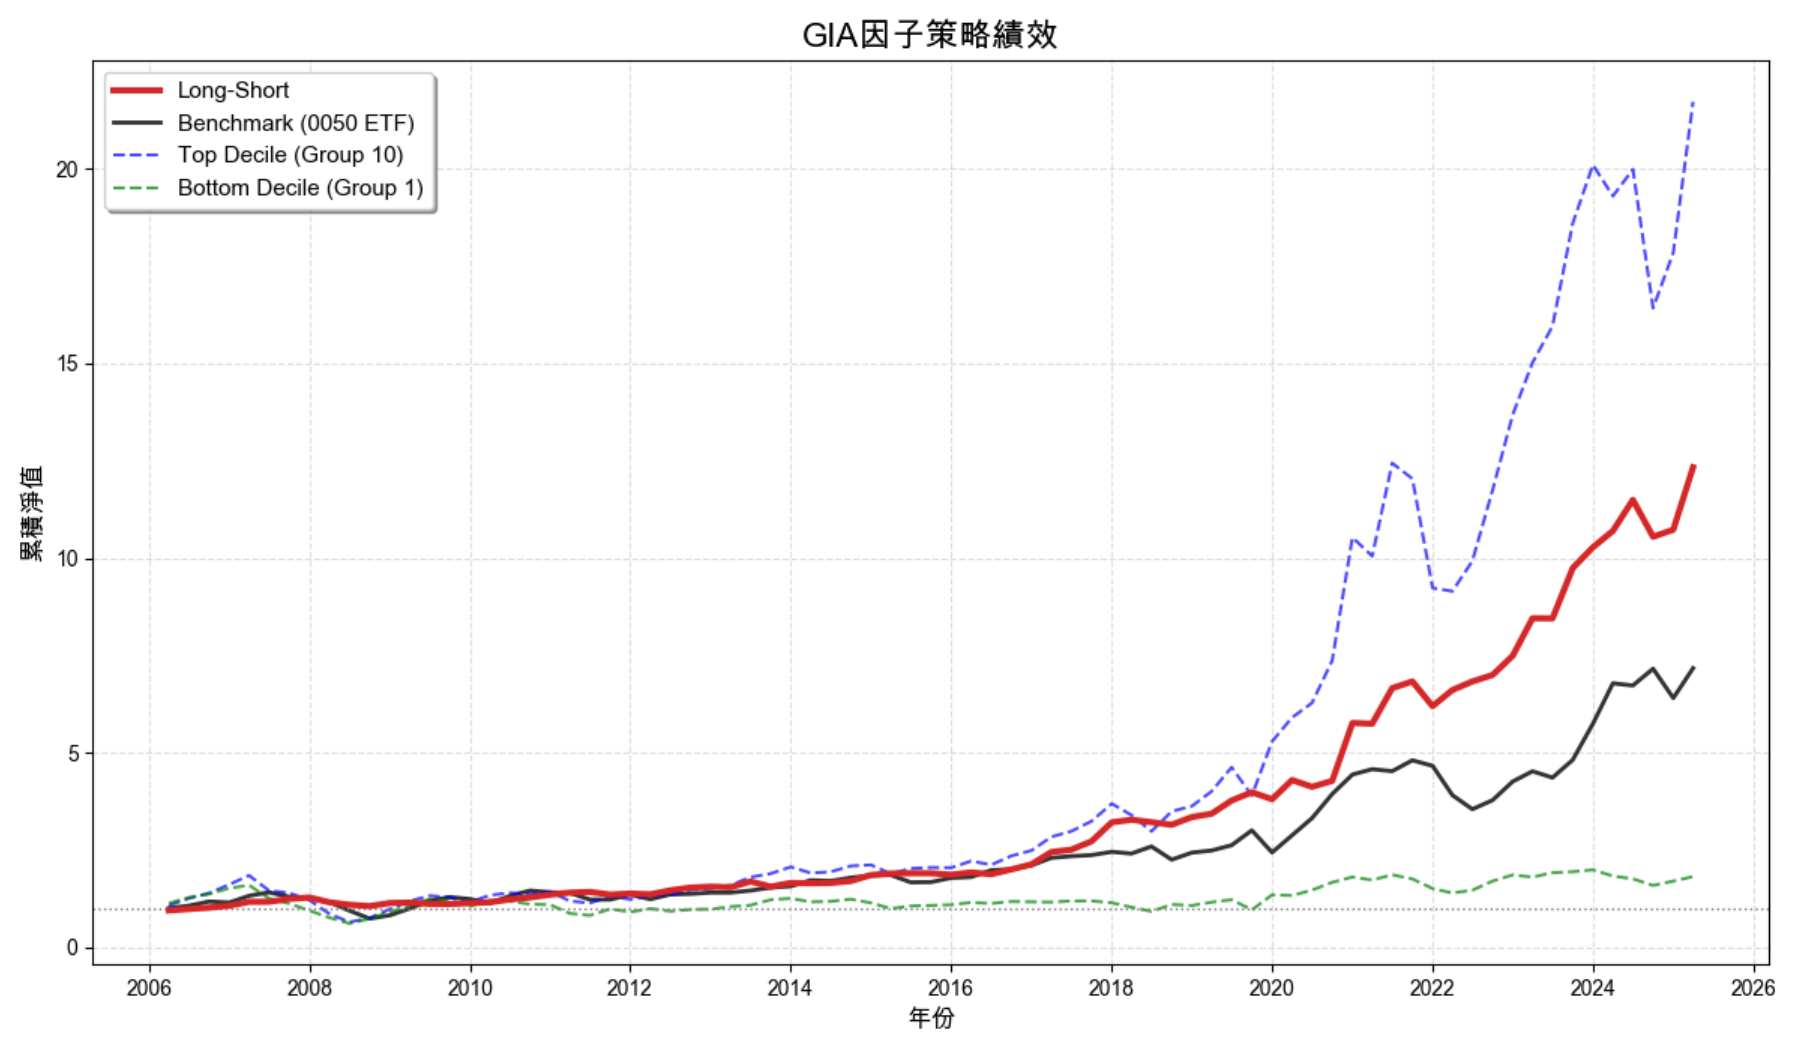
\includegraphics[width=\linewidth]{fig1_cumret.png}
\end{column}
\begin{column}{0.29\textwidth}
\small
\begin{itemize}\setlength{\itemsep}{9pt}
  \item D10 淨值展現強勁複利成長，長期大幅跑贏大盤。
  \item L/S 平穩向上，於 2008、2022 空頭僅受輕傷，展現市場中立的防禦優勢。
\end{itemize}
\end{column}
\end{columns}
\figcap{圖 1：GIA 策略（D10／D1／L/S）與 0050 ETF 累積報酬走勢。}
\end{frame}

\begin{frame}{穩健性檢定 — 風險調整後 Alpha}
\vspace{0.1cm}
\small 以 Carhart 四因子迴歸檢定各組 Jensen's Alpha：
\vspace{3pt}
\begin{center}\footnotesize
\begin{tabular}{c *{10}{c}}
\toprule
分組 & 1 & 2 & 3 & 4 & 5 & 6 & 7 & 8 & 9 & 10 \\
\midrule
$\alpha_{4F}$ & $-1.70$ & $-0.77$ & $-1.00$ & $-0.97$ & $-0.29$ & $0.19$ & $-0.16$ & $-0.86$ & $-0.10$ & $1.22$ \\
\bottomrule
\end{tabular}
\end{center}
\vspace{6pt}
\begin{itemize}\setlength{\itemsep}{6pt}
  \item \textbf{多空策略}：純粹 Alpha \hl{2.92\%}（$t=4.57$，1\% 顯著）—— 有效抵銷共同風險，提煉最純粹可信的超額報酬。
  \item \textbf{鎖定真實贏家}：D10 的 $\alpha=1.22\%$（因承擔較高波動，統計上未達顯著），但對比 0050 ETF 的\textbf{顯著負值} $\hl{-3.48\%}$，仍展現更佳的超額報酬體質與防禦性。
  \item \textbf{過濾虛假獲利}：D1 的 $\alpha=-1.70\%$，確認模型能有效識別落後股。
\end{itemize}
\end{frame}

\begin{frame}{策略相對優勢 — 與市場標竿比較}
\vspace{0.2cm}
\begin{center}\small
\textbf{表 6\ \ GIA 策略與市場標竿（0050 ETF）績效比較}\\[5pt]
\begin{tabular}{l c c c}
\toprule
績效指標 & GIA 贏家組 (D10) & GIA 多空 (L/S) & 0050 ETF \\
\midrule
年化報酬率 & \textbf{19.72\%} & 14.12\% & 12.18\% \\
總累積報酬 & \textbf{2072.60\%} & 1133.28\% & 617.02\% \\
年化波動率 & 26.40\% & \textbf{13.70\%} & 19.10\% \\
夏普比率 & 0.75 & \textbf{1.03} & 0.64 \\
最大回撤 & $-$64.95\% & \textbf{$-$17.39\%} & $-$47.81\% \\
Jensen's Alpha & 1.22\% & \textbf{2.92\%} & $-$3.48\% \\
\bottomrule
\end{tabular}
\end{center}
\vspace{6pt}
\small
\begin{itemize}\setlength{\itemsep}{4pt}
  \item \textbf{積極型（D10）}：追求成長極大化，總累積報酬達 0050 的 3.3 倍以上。
  \item \textbf{穩健型（L/S）}：低波動、高夏普（1.03 vs.\ 0.64）、低回撤，追求絕對報酬與效率。
\end{itemize}
\end{frame}

\begin{frame}{實務落地 — 交易成本與淨報酬}
\vspace{0.3cm}
\begin{itemize}\setlength{\itemsep}{10pt}
  \item \textbf{換股率}：贏家組（D10）季均單邊換股率約 \hl{73.7\%}，反映主動選股的動態調整。
  \item \textbf{成本試算（保守）}：證交稅 0.3\% + 手續費 0.1425\%（未折扣）+ 市場衝擊，設單邊 0.3\%、雙邊 0.6\%：
  \[ \text{年化成本}\approx 73.7\%\times 0.6\%\times 4 \approx \hl{1.77\%} \]
  \item \textbf{淨績效}：D10 年化原始報酬 19.72\% 扣成本後，淨報酬仍達 \hl{17.95\%}，遠勝 0050 ETF 的 12.18\%。
  \item \textbf{結論}：GIA 捕捉的 Alpha 訊號強度足以覆蓋頻繁交易成本，具高度實務投資價值。
\end{itemize}
\end{frame}

% ====================== 第五章 ======================
\chapterframe{第五章}{結論與未來展望}

\begin{frame}{研究結論總結}
\vspace{0.2cm}
\small
\begin{enumerate}\setlength{\itemsep}{8pt}
  \item \textbf{頻譜過濾有效解決維度災難}：截斷 SVD 能分離「市場共識」與「隨機雜訊」；共識型因子需高 $K$、私有資訊因子需低 $K$，為因子投資提供動態參數校準依據。
  \item \textbf{核心因子篩選與反向訊號}：Return Gap 在台股顯著負向（$t=-2.51$）源自資訊遞延的歸因錯置；經方向校準與整合，建構 6 因子 GIA 模型。
  \item \textbf{贏家組優於被動投資}：D10 年化原始 19.72\%，扣成本後淨報酬 17.95\% 仍遠勝 0050 ETF 12.18\%；對比 0050 顯著負 Alpha，主動選股實質價值更高。
  \item \textbf{多空策略驗證統計穩健性}：L/S 風險調整後 Alpha 2.92\%（1\% 顯著），證實模型能穩健區別優劣股、訊號非隨機雜訊。
\end{enumerate}
\end{frame}

\begin{frame}{管理意涵}
\vspace{0.25cm}
\begin{itemize}\setlength{\itemsep}{11pt}
  \item \textbf{對一般投資人}：被動投資扣除風險後實質侵蝕 Alpha；善用機構持股資訊，即使每季調整一次，仍能創造顯著優於大盤的財富增值。
  \item \textbf{對量化基金經理人}：GIA 提供將龐雜「機構持股」轉化為「系統性 Alpha 因子」的標準化「因子化工程」，使持股數據成為多因子模型的關鍵另類特徵。
  \item \textbf{對產品設計者}：GIA 應作為強力的「多頭篩選引擎」，以贏家清單為核心持股池、疊加波動控管，建構高爆發力且可執行的主動型產品。
\end{itemize}
\end{frame}

\begin{frame}{研究限制}
\vspace{0.25cm}
\begin{itemize}\setlength{\itemsep}{11pt}
  \item \textbf{下檔風險來自市場 Beta}：D10 最大回撤達 $-64.95\%$，但這是「純做多」在系統性崩盤下的市場特性；L/S 同期 MDD 僅 $-17.39\%$，證明高回撤源自\textbf{無法剝離的市場 Beta}，而非選股因子失效。
  \item \textbf{放空限制}：台灣有嚴格放空限制與借券成本，L/S 績效應視為\textbf{模型預測力的理論上限}（驗證訊號純度），而非完全可複製的實務報酬。
  \item \textbf{持股頻率限制}：依賴每季持股明細，Return Gap 仍屬落後性質的代理變數，無法即時反映每日持股變動。
\end{itemize}
\end{frame}

\begin{frame}{未來研究建議}
\vspace{0.25cm}
\begin{itemize}\setlength{\itemsep}{10pt}
  \item \textbf{機器學習與非線性整合}：以 Random Forest／XGBoost 取代等權重，學習 9 大因子間的非線性關係與交互作用，並依市場狀態動態調整權重。
  \item \textbf{投組優化與風險預算}：將 GIA 預測 Alpha 作為輸入，結合均值-變異數優化（MVO）或風險平價，進行風險預算以壓低尾部風險與最大回撤。
  \item \textbf{擴充輸入維度}：納入基金資金流量（聰明錢效應）等多元另類 Alpha 指標，豐富 GIA 模型的資訊含量。
  \item \textbf{主動型 ETF 應用}：GIA 數學架構高度可移植，未來可套用於每日揭露持股的主動型 ETF，在高頻維度驗證選股時效性。
\end{itemize}
\end{frame}

\begin{frame}{主要參考文獻}
\vspace{0.1cm}
\scriptsize
\begin{itemize}\setlength{\itemsep}{2.5pt}
  \item Wermers, R., Yao, T., \& Zhao, J. (2012). Forecasting stock returns through an efficient aggregation of mutual fund holdings. \textit{RFS}, 25(12).
  \item Cohen, R. B., Coval, J. D., \& Pástor, Ľ. (2005). Judging fund managers by the company they keep. \textit{JF}, 60(3).
  \item Cremers, K. J. M., \& Petajisto, A. (2009). How active is your fund manager? \textit{RFS}, 22(9).
  \item Kacperczyk, M., Sialm, C., \& Zheng, L. (2005; 2008). Industry concentration; Unobserved actions of mutual funds. \textit{JF}; \textit{RFS}.
  \item Amihud, Y., \& Goyenko, R. (2013). Mutual fund's $R^2$ as predictor of performance. \textit{RFS}, 26(3).
  \item Grinblatt, M., Titman, S., \& Wermers, R. (1995). Momentum, portfolio performance, and herding. \textit{AER}, 85(5).
  \item Elton, E. J., Gruber, M. J., \& Blake, C. R. (2011). Holdings data, security returns, and selection of superior funds. \textit{JFQA}, 46(2).
  \item Jones, C. S., \& Mo, H. (2021). Out-of-sample performance of mutual fund predictors. \textit{RFS}, 34(1).
  \item DeMiguel, V., Garlappi, L., \& Uppal, R. (2009). Optimal versus naive diversification (1/N). \textit{RFS}, 22(5).
  \item Li, Z., \& Rao, X. (2023). Exploring the zoo of predictors for mutual fund performance in China. \textit{PBFJ}, 77.
  \item 李春安、賴藝文 (2005)。股市劇烈變動區間台灣股票市場與本國機構投資人從眾行為之研究。\textit{台灣管理學刊}。
  \item 盧秋玲、張清發、沈仰斌 (2017)。積極比例是否解釋台灣共同基金績效？\textit{證券市場發展季刊}。
\end{itemize}
\end{frame}

% ====================== 結尾 ======================
\begin{frame}[plain]
\begin{tikzpicture}[remember picture,overlay]
  \fill[nccublue] (current page.north west) rectangle ([yshift=-1.12cm]current page.north east);
  \node[anchor=south east,inner sep=0pt] at ([xshift=0cm,yshift=-1.12cm]current page.north east)
    {
\includegraphics[height=1.12cm]{nccu_logo.png}};
  \node[align=center,text=ink] at (current page.center)
    {{\songti\fontsize{24}{32}\selectfont 報告結束\quad 感謝聆聽}\\[18pt]
     {\fontsize{15}{24}\selectfont 特別感謝指導教授 \textbf{羅秉政} 博士的悉心指導，}\\[6pt]
     {\fontsize{15}{24}\selectfont 以及\textbf{各位口試委員}的寶貴意見。}};
\end{tikzpicture}
\end{frame}

\end{document}
